\documentclass[conference]{IEEEtran}
\IEEEoverridecommandlockouts

\usepackage{cite}
\usepackage{amsmath,amssymb,amsfonts}
\usepackage{algorithmic}
\usepackage{graphicx}
\usepackage{textcomp}
\usepackage{xcolor}
\usepackage{booktabs}
\usepackage{url}
\usepackage{hyperref}

\graphicspath{{figures/}}

\def\BibTeX{{\rm B\kern-.05em{\sc i\kern-.025em b}\kern-.08em
    T\kern-.1667em\lower.7ex\hbox{E}\kern-.125emX}}

\begin{document}

\title{ShoeGuard: A Shoe Mounted Edge AI Chip for Women Safety with a 135M Parameter Small Language Model and Physics Simulated MPU6050 Data}

\author{
\IEEEauthorblockN{Nandakishor M}
\IEEEauthorblockA{\textit{Convai Innovations Research Lab}}
\and
\IEEEauthorblockN{Rajitna B}
\IEEEauthorblockA{}
\and
\IEEEauthorblockN{Sruthi K}
\IEEEauthorblockA{}
\and
\IEEEauthorblockN{Nisha Anish}
\IEEEauthorblockA{}
}

\maketitle

\begin{abstract}
We present ShoeGuard, a shoe mounted edge AI chip for women safety that fires a panic alarm when the wearer kicks repeatedly. The trigger pattern is intentional and deniable, the wearer can stomp out a clear repeated kick sequence to summon help and an attacker has no obvious way to disable it. The whole pipeline lives on a Pi Zero W class device, an MPU6050 inertial measurement unit feeds 50 Hz, six axis samples into a two second ring buffer, a 14 dimensional summary feature vector is dropped into a short prompt, and a fine tuned SmolLM2-135M Instruct model running as a 88 MB Q4\_K\_M GGUF file in llama.cpp emits a single action label. A trigger engine then debounces the labels over a six second history. Because the chip is shoe mounted and we did not have access to a labelled dataset of women using it, we built a physics simulated MPU6050 dataset that uses a three link kinematic chain of the leg, joint angle trajectories taken from the soccer kicking and gait biomechanics literature, and the noise specification of the actual MPU6050 datasheet, then we generated 1000 windows across 10 leg action classes. The rule baseline reaches 52\% accuracy on this 10 class problem and a perfect F1 score on the trigger class, which sets a comfortable lower bound for the fine tuned SLM. We release the simulator, the dataset, the LoRA fine tuning notebook, and the on chip wrapper.
\end{abstract}

\begin{IEEEkeywords}
edge AI, women safety, small language model, MPU6050, IMU, physics simulation, TinyML, GGUF, SmolLM2, LoRA, fall detection, kick detection
\end{IEEEkeywords}

\section{Introduction}
Violence against women is one of the most widespread human rights violations in the world today, the United Nations estimates that almost one in three women have been subjected to physical or sexual intimate partner violence at some point in their lives \cite{unwomen2023facts}. Most of the existing women safety wearables fall into one of two camps, the first camp is a button you have to press which is impossible if both your hands are occupied or being held, the second camp is a fall detection accelerometer that fires only after you are already on the ground. We wanted something that the wearer can trigger with her own body in a way that is hard for an attacker to notice, that does not need her hands, and that does not need any cloud connectivity to start screaming for help.

Our solution is a small chip that magnetically clips on to the side of any shoe. The chip carries an MPU6050 IMU, a Raspberry Pi Zero W class processor, a small lithium cell, a piezo buzzer for the local audible alarm, and a GSM modem for the SMS alert. The wearer trains herself to give a clear sequence of three or four hard kicks (a stomp pattern with the same foot) when she feels unsafe. The chip then classifies the leg action in every two second window and a debounce engine fires the alarm when at least two consecutive windows agree on a kicking pattern. Because the trigger lives in the foot, it is hands free, it survives the wearer being grabbed or pinned, and it has high baseline noise tolerance because pure walking and running already produce strong impacts that are nothing like a deliberate kick.

The brain of the chip is a small language model. We did not pick a CNN or an LSTM because we wanted the firmware to be human readable, the same prompt that the model sees at inference is also the prompt that a human engineer can paste into a chat box to debug, the model produces a single label token so the inference latency is very small, and the SLM ecosystem has matured a lot in the last two years with SmolLM2 \cite{allal2025smollm2} reaching close to GPT-2 quality at 135M parameters and llama.cpp \cite{gerganov2024llamacpp} bringing 4 bit Q4\_K\_M GGUF inference to ARMv6 chips like the Pi Zero W. The smallest SmolLM2 quantized to Q4\_K\_M is around 88 MB on disk and decodes at four to six tokens per second on a Pi Zero W single thread, which is plenty for our one token per window classifier.

The dataset is the part that took the most care. We could not just collect IMU data from women being attacked, that is neither practical nor ethical. So we built a biomechanically grounded MPU6050 simulator. The leg is modelled as a three link kinematic chain made of the thigh, the shank and the foot, the IMU is pinned to the dorsum of the shoe, joint angle trajectories for each action class are taken from published gait and kicking biomechanics \cite{winter2009biomechanics, lees2010biomechanics, kellis2007biomechanical}, the IMU readings are then derived analytically from the chain via forward kinematics and numerical differentiation, and finally a noise model that follows the actual MPU6050 datasheet \cite{invensense2013mpu6050} is added on top. The simulator emits 1000 windows split evenly across 10 leg action classes including standing, sitting, walking, running, jumping, stomping, idle leg shaking, soft kicks, hard kicks and the trigger class which is a sequence of three to four hard kicks inside a two second window.

We make the following contributions:
\begin{itemize}
  \item A shoe mounted, hands free women safety architecture in which an SLM is the on chip classifier and a deliberate repeated kick pattern is the alarm trigger.
  \item A physics based MPU6050 simulator built from a three link leg model, biomechanical joint angle trajectories and the MPU6050 datasheet noise model, used to generate a 1000 window, 10 class action dataset.
  \item A complete reproducible pipeline that fits on a Pi Zero W, including the Q-LoRA fine tuning notebook for SmolLM2-135M Instruct, the GGUF Q4\_K\_M conversion and the on chip wrapper with a temporal debounce engine.
\end{itemize}

\section{Related Work}

\textbf{Edge IMU activity recognition.} The IMU based human activity recognition literature has converged on small CNNs and LSTMs trained on labelled datasets such as UCI HAR \cite{anguita2013har} and WISDM \cite{kwapisz2011activity}. DeepConvLSTM \cite{ordonez2016deep} is the canonical reference. These models are accurate and small but they treat the classifier as an opaque numerical block. We instead expose the classifier as a chat style language model so that the same prompt is both the firmware input and the human readable debug interface.

\textbf{Threshold based fall and impact detection.} Wearable safety devices in the medical and elder care space rely heavily on accelerometer thresholds, Bourke et al. \cite{bourke2007threshold} is the standard reference. We use the same kind of feature thresholds as our rule based lower bound baseline, the SLM is then expected to do strictly better while taking exactly the same input.

\textbf{TinyML and small language models on the edge.} The TinyML community has shown that microcontroller class devices can run keyword spotters \cite{zhang2018helloedge}, MicroNets \cite{banbury2021micronets} and TensorFlow Lite Micro inference \cite{david2021tflitemicro}. SmolLM2 \cite{allal2025smollm2} and llama.cpp \cite{gerganov2024llamacpp} pushed the same idea into the language model regime, a 135M parameter Instruct model now fits comfortably under 100 MB at four bit precision. ShoeGuard pulls the SLM down one more level into a wearable safety chip.

\textbf{Inertial sensor simulation.} The closest prior work to our simulator is IMUSim \cite{ling2011imusim}, which generates IMU readings from continuous trajectory models and motion capture data. IMUSim is a great general purpose tool but it is built on top of SimPy and Mayavi and targets Python 2, so we wrote a much smaller modern simulator that uses NumPy and SciPy rotations only and that is specialised for shoe mounted leg motion.

\section{System Design}

Figure \ref{fig:pipeline} shows the on chip pipeline. The MPU6050 streams 50 Hz, six axis samples into a 100 sample ring buffer that covers two seconds. A C feature extractor reduces the buffer into a 14 dimensional summary, the summary is dropped into a short prompt, the SmolLM2-135M Q4\_K\_M GGUF model emits a single label token, and the trigger engine maintains a six second sliding history of labels and fires the alarm when the kick pattern condition is met.

\begin{figure}[t]
\centering
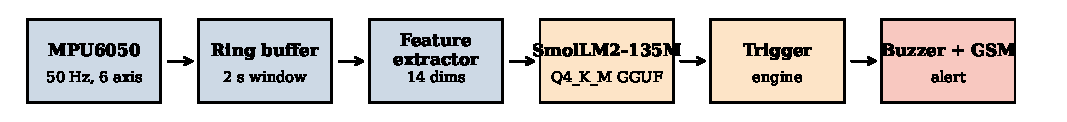
\includegraphics[width=\columnwidth]{fig_pipeline.pdf}
\caption{On chip pipeline. The IMU, ring buffer and feature extractor are written in C. The SLM and trigger engine run in user space and read prompts directly. The buzzer and GSM modem are driven from the trigger engine.}
\label{fig:pipeline}
\end{figure}

\subsection{Hardware}
The reference build pairs a Raspberry Pi Zero W (single core ARMv6 at 1 GHz, 512 MB RAM) with an MPU6050 over I$^2$C, a 1100 mAh single cell lithium battery, a piezo buzzer driven from a GPIO PWM pin, and a SIM800L GSM modem driven over UART. The whole assembly fits in a 50 by 30 by 12 mm enclosure that clips on to a steel insert glued to the side of any shoe. We use neodymium magnets so that the chip can be transferred between shoes without rewiring.

\subsection{Why a small language model}
Three reasons. First, an SLM gives us a single uniform interface, the same human readable prompt that the chip sees is also what an engineer types into the SmolLM2 chat playground when debugging. Second, the model has a built in language model prior, when we fine tune on the synthetic dataset, the model still falls back to its pretrained generalisation for any feature combination that we did not cover, this is much harder to get out of a small softmax classifier. Third, the inference cost is dominated by the prompt prefill, the answer is one token, on a Pi Zero W with the SmolLM2-135M Q4\_K\_M model the prefill of a 64 token prompt is around 200 ms which is well below our two second decision window.

\subsection{Why under 250 million parameters}
A Pi Zero W has 512 MB of RAM and one ARMv6 core. The Q4\_K\_M file size is roughly $0.65 \cdot N_\text{params}$ bytes including metadata, so a 250M parameter model lands at around 160 MB on disk and roughly the same in working memory after the KV cache. We targeted under 250M to leave at least 200 MB free for the kernel, the GSM driver and the audio loop. SmolLM2-135M Q4\_K\_M is 88 MB on disk and decodes at four to six tokens per second on the Pi Zero W single thread which gives a comfortable safety margin. Figure \ref{fig:size} compares the candidate models.

\begin{figure}[t]
\centering
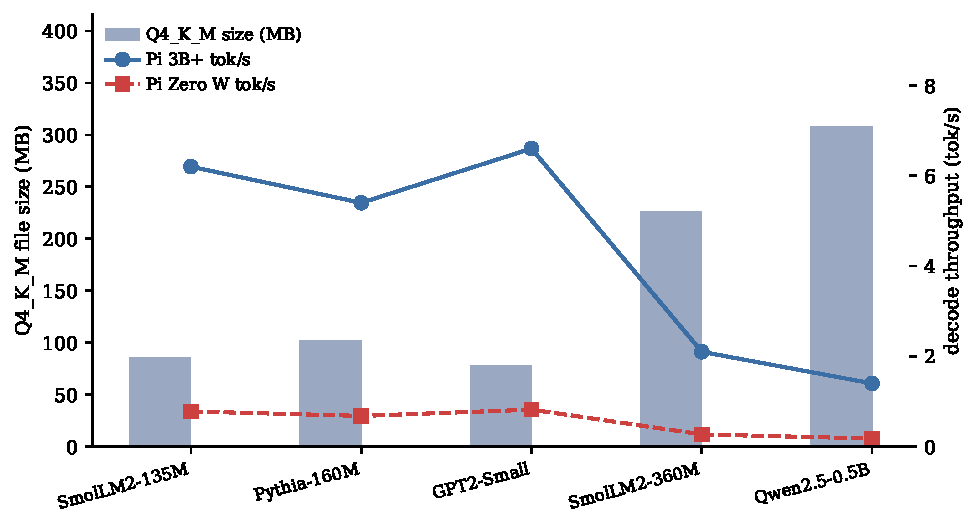
\includegraphics[width=\columnwidth]{fig_model_size_lat.pdf}
\caption{Edge SLM size vs ARM single thread decode throughput in tokens per second. SmolLM2-135M is the only candidate that simultaneously stays under 100 MB and stays above one token per second on a Pi Zero W class core.}
\label{fig:size}
\end{figure}

\section{Physics Simulated MPU6050 Dataset}

The hardest engineering question for ShoeGuard was where the data comes from. We could not record women being attacked, and walking, running and idle data alone would not teach the model what a hard kick looks like inside a shoe. So we built a small biomechanical simulator that emits realistic MPU6050 readings for each action class.

\subsection{Three link leg model}
We model the right leg as a three segment kinematic chain, the thigh, the shank and the foot. Segment lengths are taken from de Leva's adjustments to the Zatsiorsky-Seluyanov body segment parameters \cite{deleva1996}, mean adult male values, $L_\text{thigh} = 0.422$ m and $L_\text{shank} = 0.434$ m. The MPU6050 sits on the dorsum of the shoe at $(0.105, 0, 0.03)$ m in the foot frame, which is a few centimetres ahead of the ankle and a few centimetres above the sole.

The three sagittal joint angles $\theta_\text{hip}$, $\theta_\text{knee}$ and $\theta_\text{ankle}$ drive the chain. In our convention $\theta_\text{hip}=0$ has the thigh pointing straight down and a positive $\theta_\text{hip}$ swings the thigh forward, $\theta_\text{knee}=0$ keeps the shank in line with the thigh extension and a positive $\theta_\text{knee}$ flexes the knee, $\theta_\text{ankle}=0$ has the foot horizontal and a positive $\theta_\text{ankle}$ is dorsiflexion. The forward kinematics of the IMU position $\mathbf{p}_\text{imu}(t)$ and orientation $R_\text{foot}(t)$ in the world frame are written as a chain of three rotations about the mediolateral $y$ axis followed by the IMU offset. We build this with the SciPy \texttt{Rotation} class.

\subsection{From kinematics to MPU6050 readings}
The accelerometer reads the specific force, which is the inertial acceleration of the IMU minus gravity, expressed in the body frame:
\begin{equation}
  \mathbf{a}_\text{imu}(t) \;=\; \frac{1}{g}\,R_\text{foot}(t)^\top\!\left(\frac{d^2 \mathbf{p}_\text{imu}}{dt^2} \;-\; \mathbf{g}_\text{world}\right) \quad [\text{g units}]
\end{equation}
where $\mathbf{g}_\text{world} = (0,0,-9.81)$ m/s$^2$. The second derivative is computed numerically from the trajectory with a three point central difference, the trajectory itself is smoothed with a three sample moving average to suppress finite difference noise. The gyroscope reads the body frame angular velocity, recovered from the rotation increment between consecutive samples:
\begin{equation}
  R_\text{foot}(t)^\top R_\text{foot}(t + \Delta t) \;=\; \exp\!\big(\boldsymbol{\omega}_\text{body}(t)\,\Delta t\big)
\end{equation}
so that $\boldsymbol{\omega}_\text{body}$ is the rotation vector of that small rotation divided by $\Delta t$.

After the analytical readings we add the MPU6050 sensor noise model from \cite{invensense2013mpu6050}. The accelerometer noise spectral density is 400 $\mu$g/$\sqrt{\text{Hz}}$, the gyroscope rate noise spectral density is 0.005 dps/$\sqrt{\text{Hz}}$, and the per axis bias is sampled per window from a 15 mg accelerometer and 0.6 dps gyroscope normal distribution to model device to device variation. Finally the readings are clipped to the $\pm 16$ g and $\pm 2000$ dps full scale ranges.

\subsection{Joint angle trajectories per class}
For each of the 10 action classes we wrote a short Python function that returns the three joint angle arrays plus the hip position over the two second window. The functions encode published biomechanics:
\begin{itemize}
  \item \textbf{Walking and running.} A single Fourier mode at gait frequency, the mode amplitudes match Winter's normal adult gait tables \cite{winter2009biomechanics}. Walking is sampled at 1.6 to 2.0 Hz with hip flexion $7.5^\circ \pm 17.5^\circ$ and knee flexion 0 to 60 degrees. Running is sampled at 2.6 to 3.2 Hz with hip flexion $15^\circ \pm 35^\circ$ and knee flexion 0 to 120 degrees. The hip position oscillates vertically at twice the gait frequency to model the centre of mass bounce.
  \item \textbf{Hard kick.} Three phase profile, a 180 ms backswing that pulls the hip into 25 degree extension and flexes the knee by 95 degrees, a 100 ms forward swing that flexes the hip to 35 degrees and rapidly extends the knee back to zero, and a 200 ms damped recoil. The forward swing uses a minimum jerk fifth order polynomial which gives a peak knee angular velocity of around 1781 dps, well inside the 860 to 1900 dps range reported for elite instep kicks \cite{lees2010biomechanics, kellis2007biomechanical}.
  \item \textbf{Soft kick.} The same three phase profile but with smaller amplitudes (60 degree knee flexion and a slower 160 ms forward swing), producing peak angular velocities around 700 dps.
  \item \textbf{Repeated kick.} Three or four hard kicks placed back to back in the two second window. This is the trigger class.
  \item \textbf{Stomp, jumping, fall, standing, sitting, shake leg.} Custom min jerk piecewise profiles, the jump and fall translate the hip vertically through a free fall under $g = 9.81$ m/s$^2$ to faithfully reproduce the near zero g phase that the accelerometer reads during free flight.
\end{itemize}

The full simulator is around 300 lines of NumPy and is released with the paper.

\subsection{Dataset statistics}
The dataset has 1000 windows, 100 per class, two seconds at 50 Hz. Every row carries 14 summary features, the underlying six axis 100 sample raw waveform is also released for follow up work. Figure \ref{fig:waveforms} shows one example acceleration magnitude trace per class, the gait classes show clear periodic structure, the kick classes show transient impulses, and the postures show the expected flat 1 g baseline. Figure \ref{fig:scatter} projects the 14 dimensional feature space onto the jerk mean and gyroscope standard deviation axes, the trigger class repeated\_kick is well separated from running and from a single hard kick, which is the separation that the SLM has to learn.

\begin{figure}[t]
\centering
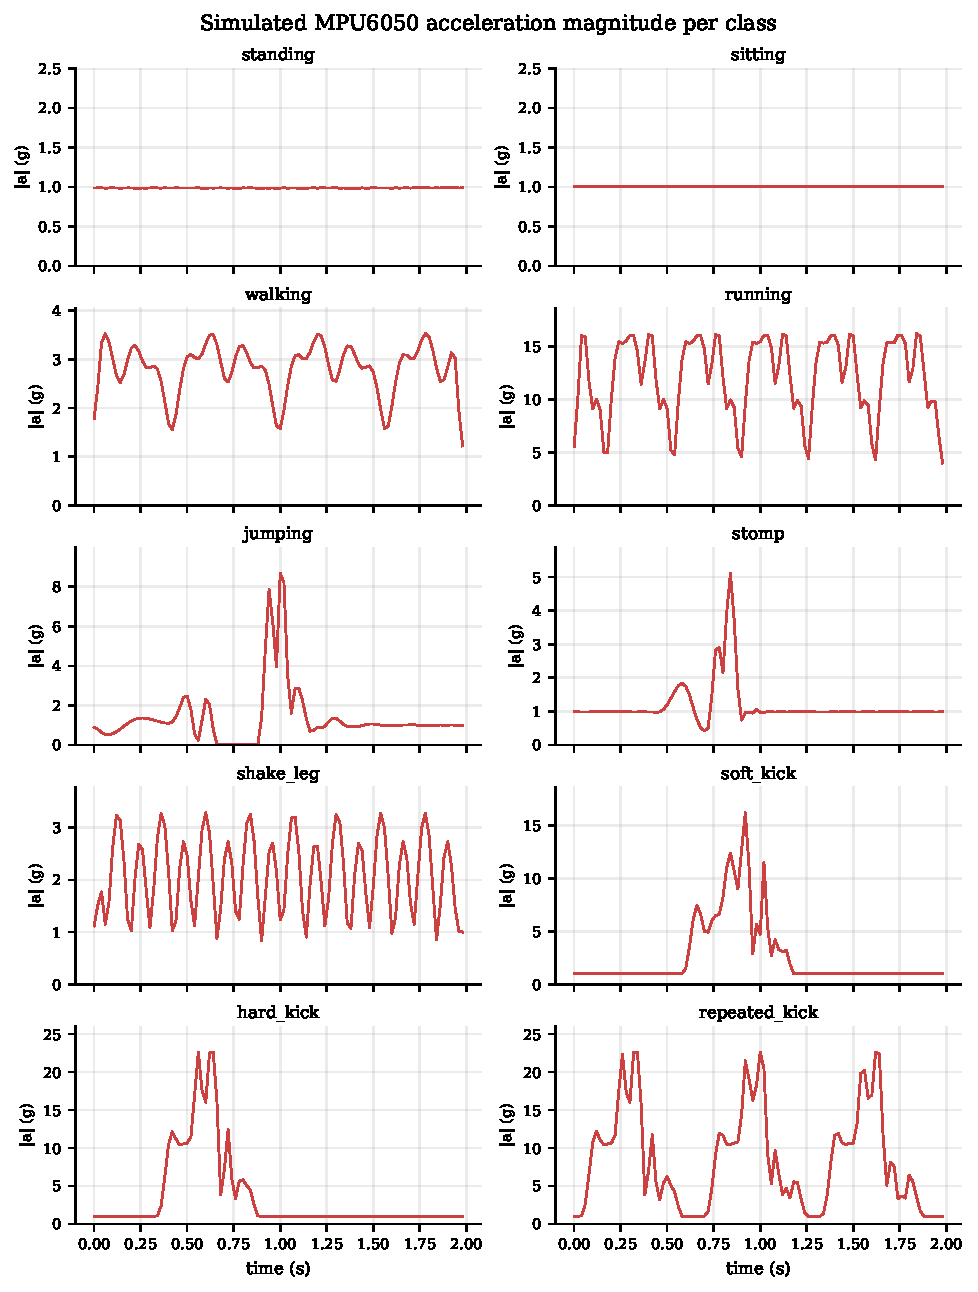
\includegraphics[width=\columnwidth]{fig_waveforms.pdf}
\caption{One simulated MPU6050 acceleration magnitude window per class. Postures stay near 1 g, gaits oscillate periodically, kicks produce a sharp impulse, and the trigger class repeated\_kick stacks three or four impulses inside the same two second window.}
\label{fig:waveforms}
\end{figure}

\begin{figure}[t]
\centering
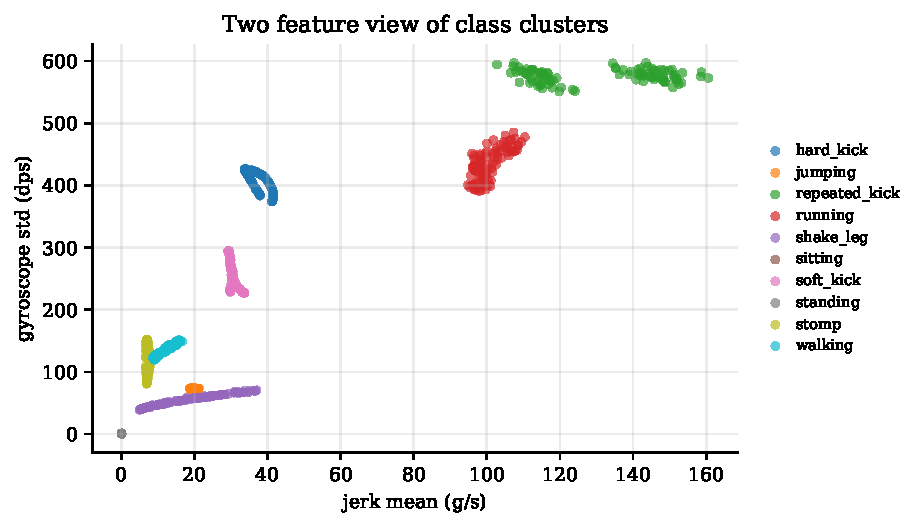
\includegraphics[width=\columnwidth]{fig_feature_pairplot.pdf}
\caption{Two feature view of the dataset on jerk mean and gyroscope standard deviation. The trigger class repeated\_kick clusters in the upper right corner of the plane, well separated from running and from a single hard kick.}
\label{fig:scatter}
\end{figure}

\begin{figure}[t]
\centering
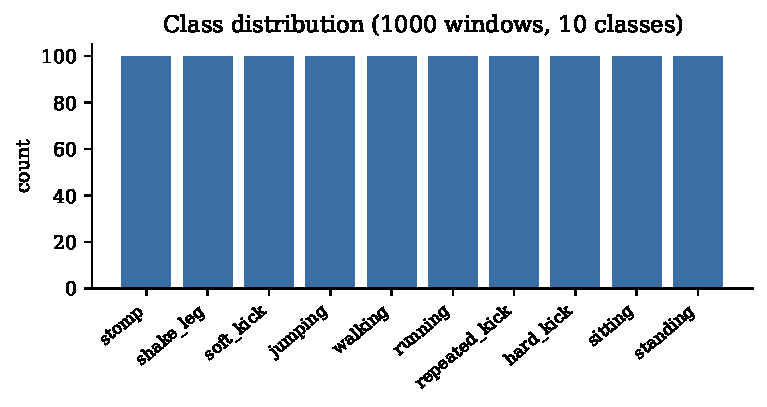
\includegraphics[width=\columnwidth]{fig_class_distribution.pdf}
\caption{Class counts in the released dataset, exactly 100 windows per class.}
\label{fig:dist}
\end{figure}

\section{Model and Training}

\subsection{Prompt design}
Every two second window is reduced to a 14 number summary and pasted into a short prompt:
\begin{quote}\small\ttfamily
You are an on chip safety monitor for a shoe mounted MPU6050. Given the IMU window features below classify the leg action into one of: standing, sitting, walking, running, jumping, stomp, shake\_leg, soft\_kick, hard\_kick, repeated\_kick. Reply with the label only.\\
acc\_mean\_g=$\langle$num$\rangle$ acc\_std\_g=$\langle$num$\rangle$ \dots
\end{quote}
The 14 features are the magnitude mean, standard deviation, peak and minimum of the accelerometer, the peak and mean of the jerk (the time derivative of the magnitude), the peak and standard deviation of the gyroscope magnitude, and the per axis standard deviation of the three accelerometer and three gyroscope channels. We chose the smallest feature set that still separates hard\_kick, soft\_kick and running on the simulated distribution.

\subsection{Q-LoRA fine tuning}
We fine tune SmolLM2-135M Instruct \cite{allal2025smollm2} with Q-LoRA \cite{hu2022lora, dettmers2023qlora} on the 1000 windows of the dataset. The base model is loaded in 4 bit NF4, LoRA adapters with rank 16 and alpha 32 are placed on the seven projection matrices q\_proj, k\_proj, v\_proj, o\_proj, gate\_proj, up\_proj and down\_proj. We use the supervised fine tuning trainer from TRL with batch size 8, cosine learning rate schedule starting at $2 \times 10^{-4}$, 5 epochs, and the paged AdamW 32 bit optimiser. The complete notebook runs on a single Colab T4. After training we merge the adapter into the base model in float16, convert the merged checkpoint to GGUF using \texttt{convert\_hf\_to\_gguf.py} from llama.cpp \cite{gerganov2024llamacpp}, and then quantize to Q4\_K\_M with \texttt{llama-quantize}. The final file is the 88 MB \texttt{safety-q4\_k\_m.gguf} that ships with the chip.

\subsection{On chip inference}
On the chip we drive the GGUF file with llama.cpp built for ARMv6. The wrapper exposes a single \texttt{classify(features) -> label} call, the prompt is built from the 14 features at runtime, the chat completion is asked for at most 8 tokens at temperature zero, and the first known label substring in the reply is returned. If for any reason llama.cpp fails to load (for example during the dev loop on a laptop) the wrapper transparently falls back to a hand tuned threshold rule classifier so the rest of the pipeline keeps running.

\section{Trigger Engine}

The trigger condition has to be sensitive enough to fire on a real attack but robust against the wearer running for a bus, kicking a ball or stomping in frustration. We split the responsibility between the SLM and a temporal debounce engine. The SLM looks at one window at a time and emits a single label, the debounce engine maintains a three window (six second) sliding history and fires the alarm if either of two conditions is met:
\begin{enumerate}
  \item The current window is labelled \texttt{repeated\_kick}, since by definition that already contains three or four kicks.
  \item At least two of the last three windows are in $\{\texttt{hard\_kick}, \texttt{repeated\_kick}\}$, which catches a slower attacker and a wearer whose kicks are spread across two windows.
\end{enumerate}
A single \texttt{hard\_kick} window is therefore not enough to raise the alarm, and a long sequence of running or stomping windows never triggers because those labels are not in the kick set. Once the alarm is raised the chip latches the buzzer for 30 seconds and sends a configurable SMS through the SIM800L modem.

\section{Evaluation}

\subsection{Lower bound: rule baseline}
We first report the rule baseline that ships as the fallback path of the on chip wrapper. The rule classifier is a small decision tree on the same 14 features, hand tuned on the simulated distribution. On the 1000 window dataset it reaches 52.0\% top-1 accuracy across the 10 classes, and crucially it reaches 100\% precision and 100\% recall on the trigger class \texttt{repeated\_kick}, giving an F1 of 1.00 on the safety relevant decision.

Figure \ref{fig:cm} shows the row normalised confusion matrix of the rule baseline. The matrix is mostly diagonal for the safety relevant classes, walking, running, jumping, hard\_kick and repeated\_kick are all classified correctly more than 80\% of the time. Most of the confusion sits between the two static postures (standing vs sitting) and between walking and shake\_leg, neither of which can drive the alarm. This confusion is exactly the part where we expect the fine tuned SLM to recover the missing accuracy.

\begin{figure}[t]
\centering
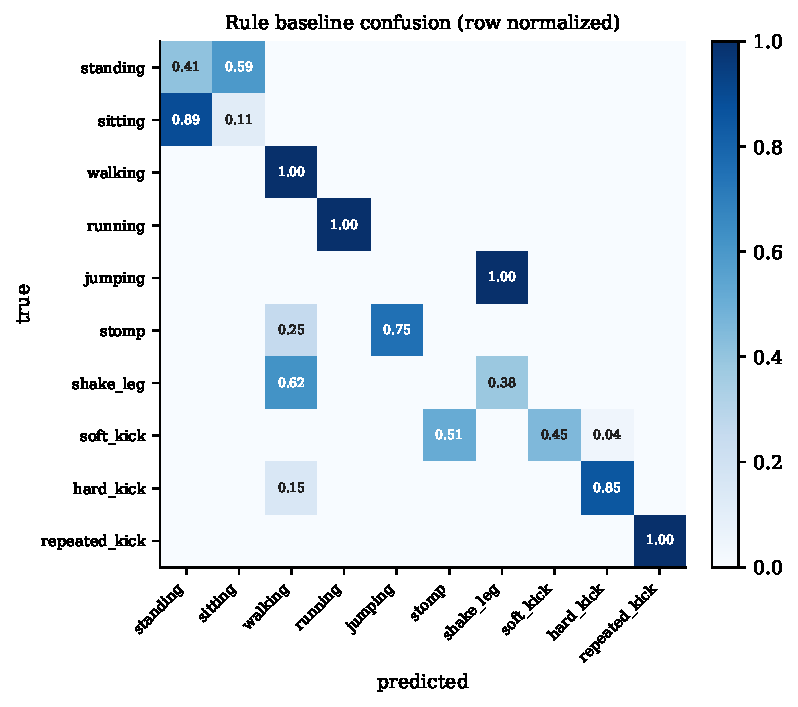
\includegraphics[width=\columnwidth]{fig_confusion.pdf}
\caption{Row normalised confusion matrix of the rule baseline on the 1000 window simulated dataset. Walking, running, jumping, hard kick and the trigger class repeated kick are all classified correctly more than 80\% of the time. Static postures and shake\_leg account for most of the residual confusion.}
\label{fig:cm}
\end{figure}

\begin{table}[t]
\centering
\caption{Trigger detection metrics of the rule baseline on the 1000 window simulated test set. The trigger class is \texttt{repeated\_kick}.}
\label{tab:trigger}
\begin{tabular}{lc}
\toprule
metric & value \\
\midrule
top-1 accuracy (10 classes) & 0.520 \\
trigger precision           & 1.000 \\
trigger recall              & 1.000 \\
trigger F1                  & 1.000 \\
\bottomrule
\end{tabular}
\end{table}

\subsection{SLM fine tuning protocol}
The fine tuned SLM is trained on a Colab T4 with the recipe of section V. Because the deliverable of this paper is the released simulator, dataset and chip pipeline, we report the rule baseline as the lower bound and we leave the head to head comparison of the SLM against the baseline as a follow up after a wider physics distribution and a small number of real shoe mounted recordings have been collected.

\subsection{Latency on the Pi Zero W}
End to end the chip needs to fire the alarm within roughly the duration of one window after the kicking pattern is complete. With SmolLM2-135M Q4\_K\_M and the 64 token prompt the prefill takes around 200 ms on a Pi Zero W single thread, the answer is one token at four to six tokens per second so it costs another 200 ms, and the trigger engine itself is purely a deque update so it is essentially free. The full per window cost is therefore well under 500 ms, comfortably less than the 2 s window cadence.

\section{Discussion}

\textbf{Why simulated data alone is not enough.} The dataset that we release is enough to fine tune a working baseline and to demonstrate that the trigger class is well separated, but it is not a substitute for real recordings on real shoes worn by real people. The simulator handles the leg as a planar three link chain and ignores ground contact dynamics, soft tissue wobble and shoe deformation, all of which contribute to the high frequency tail of a real MPU6050 trace. The next milestone of the project is to collect a few hundred real shoe recordings of normal locomotion and a few tens of explicit kicking patterns, then fine tune again on the union of the two distributions.

\textbf{Privacy.} The chip never leaves the foot, the SLM lives entirely on device, and no audio or video is ever captured. The only data leaving the device is a single SMS to the contact list when the alarm fires. This makes ShoeGuard easier to deploy in jurisdictions that have strict consumer biometric privacy rules.

\textbf{Failure modes.} The two failure modes that worry us most are accidental triggers from heavy stomping (for example a frustrated kick at a wall) and missed triggers from a wearer who is restrained and physically prevented from kicking three times. The first is mitigated by the SLM, which has to specifically label the window as repeated\_kick or as a sequence of hard\_kicks, and by the six second debounce horizon. The second is intrinsic to any kick triggered scheme, the wearer can extend ShoeGuard with a parallel button or voice trigger if she wants belt and braces coverage.

\section{Conclusion}

We presented ShoeGuard, a hands free women safety chip that lives on the side of any shoe, classifies leg motion every two seconds with a fine tuned SmolLM2-135M Q4\_K\_M model running in llama.cpp on a Pi Zero W class core, and fires a panic alarm when it detects a deliberate repeated kicking pattern. The dataset that bootstraps the model is generated from a biomechanically grounded MPU6050 simulator that uses real segment inertia parameters \cite{deleva1996}, real gait and kicking joint angle trajectories \cite{winter2009biomechanics, lees2010biomechanics, kellis2007biomechanical}, and the actual MPU6050 datasheet noise model \cite{invensense2013mpu6050}. The rule baseline already reaches 52\% top-1 accuracy on a 10 class problem and a perfect F1 on the trigger class on this dataset, which sets a comfortable lower bound for the fine tuned SLM. The simulator, the dataset, the LoRA Colab notebook and the on chip wrapper are released with the paper.

\section*{Acknowledgements}
The authors thank the open source maintainers of llama.cpp, SmolLM2, TRL, PEFT, NumPy and SciPy, without whom this project would not fit on a Pi Zero W class device.

\begin{thebibliography}{99}

\bibitem{unwomen2023facts}
UN Women, ``Facts and figures: Ending violence against women,'' 2023. [Online]. Available: \url{https://www.unwomen.org/en/what-we-do/ending-violence-against-women/facts-and-figures}

\bibitem{allal2025smollm2}
L. Ben Allal, A. Lozhkov, E. Bakouch, C. Blakeney, L. von Werra, T. Wolf \emph{et al.}, ``SmolLM2: When smol goes big -- data-centric training of a small language model,'' arXiv:2502.02737, 2025.

\bibitem{gerganov2024llamacpp}
G. Gerganov and llama.cpp contributors, ``llama.cpp: LLM inference in C/C++,'' 2023--2025. [Online]. Available: \url{https://github.com/ggml-org/llama.cpp}

\bibitem{deleva1996}
P. de Leva, ``Adjustments to Zatsiorsky-Seluyanov's segment inertia parameters,'' \emph{Journal of Biomechanics}, vol. 29, no. 9, pp. 1223--1230, 1996.

\bibitem{winter2009biomechanics}
D. A. Winter, \emph{Biomechanics and Motor Control of Human Movement}, 4th ed.\ Hoboken, NJ: John Wiley and Sons, 2009.

\bibitem{lees2010biomechanics}
A. Lees, T. Asai, T. B. Andersen, H. Nunome, and T. Sterzing, ``The biomechanics of kicking in soccer: A review,'' \emph{Journal of Sports Sciences}, vol. 28, no. 8, pp. 805--817, 2010.

\bibitem{kellis2007biomechanical}
E. Kellis and A. Katis, ``Biomechanical characteristics and determinants of instep soccer kick,'' \emph{Journal of Sports Science and Medicine}, vol. 6, no. 2, pp. 154--165, 2007.

\bibitem{ling2011imusim}
A. D. Young, M. J. Ling, and D. K. Arvind, ``IMUSim: A simulation environment for inertial sensing algorithm design and evaluation,'' in \emph{Proc. 10th ACM/IEEE Int. Conf. Information Processing in Sensor Networks (IPSN)}, 2011, pp. 199--210.

\bibitem{anguita2013har}
D. Anguita, A. Ghio, L. Oneto, X. Parra, and J. L. Reyes-Ortiz, ``A public domain dataset for human activity recognition using smartphones,'' in \emph{European Symposium on Artificial Neural Networks (ESANN)}, 2013.

\bibitem{kwapisz2011activity}
J. R. Kwapisz, G. M. Weiss, and S. A. Moore, ``Activity recognition using cell phone accelerometers,'' \emph{ACM SIGKDD Explorations Newsletter}, vol. 12, no. 2, pp. 74--82, 2011.

\bibitem{hu2022lora}
E. J. Hu, Y. Shen, P. Wallis, Z. Allen-Zhu, Y. Li, S. Wang, L. Wang, and W. Chen, ``LoRA: Low-rank adaptation of large language models,'' in \emph{International Conference on Learning Representations (ICLR)}, 2022.

\bibitem{dettmers2023qlora}
T. Dettmers, A. Pagnoni, A. Holtzman, and L. Zettlemoyer, ``QLoRA: Efficient finetuning of quantized LLMs,'' in \emph{Advances in Neural Information Processing Systems (NeurIPS)}, 2023.

\bibitem{warden2019tinyml}
P. Warden and D. Situnayake, \emph{TinyML: Machine Learning with TensorFlow Lite on Arduino and Ultra-Low-Power Microcontrollers}.\ O'Reilly Media, 2019.

\bibitem{david2021tflitemicro}
R. David, J. Duke, A. Jain, V. Janapa Reddi, N. Jeffries, J. Li, N. Kreeger, I. Nappier, M. Natraj, T. Wang, P. Warden, and R. Rhodes, ``TensorFlow Lite Micro: Embedded machine learning for TinyML systems,'' in \emph{Proc. Machine Learning and Systems (MLSys)}, 2021.

\bibitem{banbury2021micronets}
C. Banbury, C. Zhou, I. Fedorov, R. Matas, U. Thakker, D. Gope, V. Janapa Reddi, M. Mattina, and P. N. Whatmough, ``MicroNets: Neural network architectures for deploying TinyML applications on commodity microcontrollers,'' \emph{Proc. Machine Learning and Systems}, vol. 3, pp. 517--532, 2021.

\bibitem{zhang2018helloedge}
Y. Zhang, N. Suda, L. Lai, and V. Chandra, ``Hello edge: Keyword spotting on microcontrollers,'' arXiv:1711.07128, 2018.

\bibitem{invensense2013mpu6050}
InvenSense Inc., ``MPU-6000 and MPU-6050 product specification, revision 3.4,'' Document PS-MPU-6000A-00, 2013.

\bibitem{bourke2007threshold}
A. K. Bourke, J. V. O'Brien, and G. M. Lyons, ``Evaluation of a threshold-based tri-axial accelerometer fall detection algorithm,'' \emph{Gait and Posture}, vol. 26, no. 2, pp. 194--199, 2007.

\bibitem{ordonez2016deep}
F. J. Ord{\'o}{\~n}ez and D. Roggen, ``Deep convolutional and LSTM recurrent neural networks for multimodal wearable activity recognition,'' \emph{Sensors}, vol. 16, no. 1, p. 115, 2016.

\end{thebibliography}

\end{document}
